\documentclass[sigconf,nonacm]{acmart}

% ----------------------------------------------------------------------------
% We are Trapped in RAR — Overleaf-ready manuscript
% Format: ACM SIGCONF (the standard for FAccT, AIES, CHI alt.chi)
%
% [nonacm] disables ACM-specific copyright/CCS requirements while keeping
% the layout. Remove it before submitting to an actual ACM venue.
% ----------------------------------------------------------------------------

\usepackage{booktabs}
\usepackage{microtype}
\usepackage{amsmath}
\usepackage{xcolor}
\usepackage{tikz}
\usetikzlibrary{arrows.meta, positioning, calc, shapes.geometric}
\usepackage{hyperref}
\hypersetup{
  colorlinks=true,
  linkcolor=black,
  urlcolor=blue!60!black,
  citecolor=black,
}

\setcopyright{none}
\settopmatter{printacmref=false}
\renewcommand\footnotetextcopyrightpermission[1]{}
\pagestyle{plain}

% Custom epigraph environment (lightweight — avoids extra package)
\newenvironment{epigraphquote}{%
  \begin{quote}\itshape\small
}{%
  \end{quote}
}

\title{We Are Trapped in RAR}
\subtitle{How Human Selection Hardens Generative AI Bias}

\author{Prithweeraj Acharjee Porag}
\affiliation{%
  \institution{University of Toledo}
  \city{Toledo}\state{OH}\country{USA}
}
\email{pporag@rockets.utoledo.edu}

\author{Afroza Nowshin}
\affiliation{%
  \institution{University of Toledo}
  \city{Toledo}\state{OH}\country{USA}
}

\author{Antardip Himel}
\affiliation{%
  \institution{University of Toledo}
  \city{Toledo}\state{OH}\country{USA}
}
% TODO: confirm Antardip's preferred contact email and add \email{...} here.

\renewcommand{\shortauthors}{Acharjee Porag, Nowshin, and Himel}

\begin{document}

\begin{abstract}
Every time you choose the AI's default image of a CEO, you cast a vote for what the next model will believe a CEO looks like. Generative AI is known to produce demographically biased outputs, and recursive self-training is known to cause representational collapse --- yet both literatures treat the human as a passive surface. We argue the human is the \emph{active} mechanism by which generative bias is amplified across model generations.

We introduce \textbf{Recursive Aesthetic Reinforcement (RAR)}: a four-stage loop in which (1) models produce stereotyped outputs, (2) humans recognize them as representative, (3) humans redistribute them, and (4) the redistribution is reingested into the next training corpus through curation pipelines (aesthetic-score filters, popularity ranking, RLHF reward data).

A pilot (\(n=20\) DALL$\cdot$E~3 images, \(n=17\) participants) supports stages 1--2: every leadership prompt produced male-coded, white-presenting outputs (100\%); participants recognized DALL$\cdot$E defaults as ``representative'' 71\% of the time for CEO (\(p=.0001\), OR\,=\,7.20, Bonferroni-surviving). The effect is demographically contingent: male participants chose DALL$\cdot$E defaults 3$\times$ as often as female participants (Cohen's \(d=1.48\)).

We then operationalize stage 4 against \textbf{LAION-Aesthetics V2} --- a deployed instance of \emph{human-rated $\to$ predictor-filtered $\to$ model-trained} that produced Stable Diffusion's training corpus. Across 13 occupations, three aesthetic-score thresholds, and 22{,}500 image classifications via DeepFace on a Kaggle P100, we find that aesthetic filtering produces \textbf{Bonferroni-significant} demographic redistribution for \emph{three} occupations (\textbf{teacher}, \(p=1.5\!\times\!10^{-5}\); \textbf{nurse}, \(p=1.6\!\times\!10^{-4}\); \textbf{leader}, \(p=7.1\!\times\!10^{-4}\)) and null effects for the other ten. Aesthetic-variance narrowing (\(\sigma^2_{\text{filtered}}/\sigma^2_{\text{baseline}}\)) is also occupation-specific: 0.49--0.67 for most leadership and care roles, but \(\geq 1.0\) for \emph{doctor}, \emph{scientist}, and \emph{nurse} --- in those cases the filter does not narrow the visual distribution and in some cases widens it.

\textbf{Stage 4 of RAR is occupation-conditional, not universal.} The aesthetic-curation step amplifies demographic stereotypes for a specific class of role (loosely-coded care and middle-tier leadership) and is silent for others (already-tightly-stereotyped CEO/founder/executive at one extreme, and visually heterogeneous STEM roles at the other). This is a stronger and more falsifiable claim than the original framework allowed.

We close with three platform-level interventions and propose RAR as a research program connecting fairness, model collapse, recommender feedback, and human--AI co-evolution.
\end{abstract}

\keywords{generative AI, representational bias, model collapse, human-in-the-loop, fairness, feedback loops, dataset curation, LAION-Aesthetics}

\maketitle

% ============================================================================
\section{Introduction: the loop nobody named}

\begin{epigraphquote}
The danger is not that the model is broken. The danger is that the model works exactly as intended, and what it does is shrink the space of seeable images, year over year.
\end{epigraphquote}

Two literatures meet in this paper, and a third --- the one in between --- does not yet exist.

The first literature is \emph{representational bias measurement} in generative models. Bianchi et al.~\cite{bianchi2023easily} showed that text-to-image systems systematically overproduce stereotypical demographic patterns when given neutral prompts. Luccioni, Akiki, Mitchell, and Jernite~\cite{luccioni2023stable} replicated this at scale across DALL$\cdot$E~2, Stable Diffusion v1.4, and v2, documenting overrepresentation of whiteness and masculinity across 96{,}000 generated images. Naik and Nushi~\cite{naik2023social}, Raza et al.~\cite{raza2025prompting}, and the SB-Bench team~\cite{sbbench2025} extended this to occupations, personality traits, geography, and visually grounded tasks. The conclusion across this body of work is consistent: today's generative models, when prompted neutrally, produce outputs that match the stereotypes embedded in their training data.

The second literature is \emph{model collapse}. Shumailov et al.~\cite{shumailov2024curse} showed mathematically and empirically that when generative models are trained recursively on their own outputs, the resulting distribution narrows: rare modes vanish, tails are lost, the model converges to a degenerate region of the original distribution. Gerstgrasser et al.~\cite{gerstgrasser2024inevitable} showed that \emph{accumulating} real and synthetic data prevents collapse, identifying the substitution-versus-accumulation distinction as load-bearing. Drayson et al.~\cite{drayson2025detection} and Zhu et al.~\cite{zhu2024synthesize} extended this to text. Adapala~\cite{adapala2025antiouroboros}, in \emph{The Anti-Ouroboros Effect}, showed that selective feedback --- keeping only high-quality outputs --- can \emph{reverse} collapse under specific conditions.

These two literatures coexist without speaking to one another. The first asks: \emph{what biases does the model produce?} The second asks: \emph{what happens when the model trains on its own outputs?} Both leave the human out --- or treat them only as the recipient of biased outputs.

But humans are not passive. The DALL$\cdot$E image of ``a CEO'' does not stay on OpenAI's servers. It is downloaded, posted to Twitter, embedded in slide decks, scraped into LAION-Aesthetics, used to fine-tune a hundred Stable Diffusion forks, surfaced in a Pinterest board that becomes part of the next crawl. \textbf{Each of those steps is a human decision}, and each one biases the surface from which the next model will learn. The loop is not \emph{machine self-training}. It is \emph{machine output \(\rightarrow\) human selection \(\rightarrow\) public surface \(\rightarrow\) training data}. The human is the bridge.

We name this loop \textbf{Recursive Aesthetic Reinforcement (RAR)}.

\begin{figure}[t]
\centering
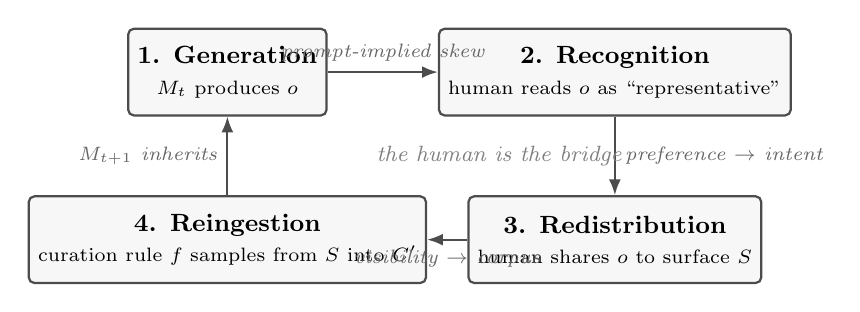
\begin{tikzpicture}[
  node distance=10mm and 14mm,
  every node/.style={font=\small},
  stage/.style={
    rectangle, rounded corners=2pt,
    draw=black!70, thick,
    minimum width=24mm, minimum height=11mm,
    align=center, fill=black!3,
  },
  flow/.style={-{Latex[length=2mm]}, thick, draw=black!70},
  label/.style={font=\scriptsize\itshape, text=black!60},
]
  \node[stage] (s1) {\textbf{1. Generation}\\\scriptsize $M_t$ produces $o$};
  \node[stage, right=of s1] (s2) {\textbf{2. Recognition}\\\scriptsize human reads $o$ as ``representative''};
  \node[stage, below=of s2] (s3) {\textbf{3. Redistribution}\\\scriptsize human shares $o$ to surface $S$};
  \node[stage, below=of s1] (s4) {\textbf{4. Reingestion}\\\scriptsize curation rule $f$ samples from $S$ into $C'$};

  \draw[flow] (s1) -- (s2) node[midway, above, label] {prompt-implied skew};
  \draw[flow] (s2) -- (s3) node[midway, right, label] {preference $\to$ intent};
  \draw[flow] (s3) -- (s4) node[midway, below, label] {visibility $\to$ corpus};
  \draw[flow] (s4) -- node[midway, left, label] {$M_{t+1}$ inherits} (s1);

  \node[font=\footnotesize, text=black!50] at ($(s1)!0.5!(s3) + (10mm, 0)$) {\emph{the human is the bridge}};
\end{tikzpicture}
\caption{The four stages of Recursive Aesthetic Reinforcement. The model generates a stereotyped output; a human recognizes it as representative; the human redistributes it to a public surface; a curation rule (aesthetic-score filter, popularity ranker, RLHF reward dataset) reingests it into the next training corpus. Each cycle compresses the representational distribution. Without the human steps (2 and 3), the loop does not close; this is the differentiator from prior automatic-self-training accounts of model collapse.}
\label{fig:rar-loop}
\end{figure}

The diagram in Figure~\ref{fig:rar-loop} makes the central claim visible: the loop is closed not by self-training in isolation, but by human selection acting on model outputs that then re-enter the training pipeline through curation. Remove stage 2 or 3, and the dynamic vanishes.

The contribution of this paper is threefold:

\begin{enumerate}
  \item \textbf{Theoretical:} A four-stage decomposition of the human-mediated bias-amplification loop, falsifiable at each stage independently, with explicit operational definitions of ``selection'' and the data pathways through which selections reach training data.
  \item \textbf{Empirical, stages 1--3:} A pilot study with 100\% inter-annotator agreement on output coding, a 17-participant forced-choice recognition task with Bonferroni-corrected significance for the CEO and Nurse prompts, and the discovery that participant gender modulates the effect with Cohen's \(d = 1.48\) --- the loop is real but breakable.
  \item \textbf{Empirical, stage 4 (novel):} The first operationalization of ``human selection reaching training data'' by analyzing LAION-Aesthetics V2 --- a public dataset whose construction is, by design, a deployed instance of stage 4 (human aesthetic ratings \(\rightarrow\) trained predictor \(\rightarrow\) curated subset \(\rightarrow\) fine-tuning corpus for downstream image generators).
\end{enumerate}

Where Bender et al.~\cite{bender2021dangers} warned about parrots that produce language without understanding, we describe a tighter, more recursive harm. The danger is not that the model knows nothing. The danger is that the model knows the user too well, and the user knows the model too well, and what they share is a narrowing of what is possible to depict.

% ============================================================================
\section{Related work: what RAR is not}

RAR sits inside an active 2024--2026 literature on AI--human feedback dynamics. It is essential to differentiate it from each adjacent framework, because surface descriptions can collapse them all into ``AI bias is amplified.'' They are not the same thing.

\textbf{Source Echo Chamber}~\cite{zhou2024source} describes how AI-generated content integrated into recommender systems creates source bias --- the recommender increasingly promotes AI-generated over human-generated content. The mechanism is the recommender's relevance score; the human acts only as a click-target. RAR operates one layer deeper: it concerns \emph{what enters training data}, not \emph{what gets shown}. A recommender bias can be debiased at the ranking layer; a RAR bias is baked into the next model's prior.

\textbf{The Lock-in Hypothesis}~\cite{qiu2025lockin} uses agent-based simulation and GPT usage data to argue that LLM use causes \emph{belief} convergence --- users come to hold a narrower set of opinions because they consult a model whose outputs are themselves narrowing. The mechanism is epistemic; the empirical surface is user belief. RAR's mechanism is curatorial-redistributive, and the surface is the training corpus itself.

\textbf{The Anti-Ouroboros Effect}~\cite{adapala2025antiouroboros} shows that \emph{selective} recursive feedback --- keeping only high-quality outputs --- can yield resilience rather than collapse. This is structurally adjacent to RAR's stage 3, but the selection criterion in Anti-Ouroboros is \emph{quality} (a normatively neutral term); in RAR, the selection criterion is \emph{stereotype-consonance} (normatively non-neutral). Anti-Ouroboros says selective feedback can preserve \emph{something}; RAR predicts it preserves the \emph{wrong} something.

\textbf{Aesthetic Alignment Risks Assimilation}~\cite{guo2025aesthetic} is the closest competitor. They show that reward models trained for aesthetic alignment systematically refuse anti-aesthetic outputs, reducing user autonomy and aesthetic diversity. The mechanism is reward-model--side suppression. RAR locates the mechanism one step earlier: in the human selections that train the reward model in the first place. Guo et al. show the \emph{consequence}; RAR names the \emph{cause}.

\textbf{Stable Bias}~\cite{luccioni2023stable} is the largest empirical foundation for our stage 1, but it is a static measurement: it characterizes the bias \emph{at one model snapshot}. RAR is the dynamic complement: it predicts how that snapshot becomes the next snapshot's prior.

\textbf{Bender et al.'s Stochastic Parrots}~\cite{bender2021dangers} --- our framing is in dialogue with this lineage. Parrots warned that scale alone does not produce understanding. RAR warns that \emph{closing the loop} between users and models does not produce diversity --- it produces convergence. The two papers describe different harms in the same general family of ``what happens when we treat statistical reflection as if it were knowledge.''

% ============================================================================
\section{The RAR framework}

We define RAR formally as a four-stage process. Each stage admits an independent empirical test; each can be falsified without disconfirming the others.

\textbf{Stage 1 --- Generation.} A generative model \(M\) produces an output \(o \sim M(p)\) for prompt \(p\). We claim \(o\) is biased iff its conditional distribution over a relevant attribute (e.g., gender, race, occupation framing) differs from the prompt-implied distribution by a measurable margin.

\textbf{Stage 2 --- Recognition.} Given \(o\) and a set of plausible alternatives \(A = \{a_1, \dots, a_n\}\), a human evaluator \(h\) selects the option they judge ``most representative'' of the prompt. We claim recognition bias exists iff \(\Pr(h\ \text{selects}\ o \mid o \in A) > 1/(|A|+1)\) significantly above chance.

\textbf{Stage 3 --- Redistribution.} A user \(u\) decides whether to share, embed, or otherwise propagate \(o\) through a public surface \(S\) (social media, blog, slide deck, image search). We define the \emph{redistribution rate} as \(R(o, u) = \Pr(u\ \text{places}\ o\ \text{on}\ S \mid u\ \text{observes}\ o)\). We claim RAR-style amplification exists iff \(R\) is positively correlated with stereotype-conformity.

\textbf{Stage 4 --- Reingestion.} A future training corpus \(C'\) is constructed by sampling from the public surface \(S\) according to some curation rule \(f\) (aesthetic-score filter, popularity-based crawling, reward-model-driven RLHF). We claim the loop closes iff items selected by \(f\) are over-representative of the stereotype distribution observed in stage 1, relative to the unfiltered baseline. (Stage 4 is operationalized empirically in Section~\ref{sec:stage4} via LAION-Aesthetics V2.)

The full loop is closed when \(M_{t+1}\) trained on \(C'\) produces stage-1 outputs that are \emph{more} stereotype-aligned than \(M_t\). We do not test the closure of the loop in this paper; we provide the first measurement of the conditional that makes closure possible (the stage-4 selection).

\textbf{Falsifiability per stage.} Stage 1 is falsified if neutrally-prompted outputs match prompt-implied distribution (within statistical noise). Stage 2 is falsified if \(\Pr(h\ \text{selects}\ o)\) does not exceed chance. Stage 3 is falsified if \(R(o,u)\) is uncorrelated with stereotype conformity. Stage 4 is falsified if curation-pipeline outputs are not stereotype-amplifying relative to baseline. Falsification of any stage \emph{does not} falsify the others --- RAR is a chain of conditional claims, not a monolithic hypothesis.

\textbf{Operationalizing ``reaches training data.''} The phrase ``redistribution is reingested into training data'' is precise only when the data pathway is named. In this paper a redistribution counts as ``reaching training data'' iff it appears on a public surface \(S\) that is included in any major training-corpus crawl (LAION, Common Crawl, the Pile-v2, RedPajama, RLHF preference datasets such as those used in Anthropic's HH-RLHF). We do not measure inclusion rates per pathway --- the upstream crawlers do not publish them --- we observe that LAION-Aesthetics V2 is one such pathway, and one whose construction we can audit (Section~\ref{sec:stage4}). Other pathways (Pinterest scrapes, Twitter image embeddings, RLHF preference data) remain available for the same operationalization in future work.

\textbf{On the ``Aesthetic'' in RAR.} The pilot study tested demographic-stereotypical content (CEO=male/white/suit/office), which is not strictly an aesthetic claim. We retain ``Aesthetic Reinforcement'' because the \emph{mechanism} --- preference-driven recursive selection --- is the same one that operates on aesthetic dimensions (composition, color, polish), and stage 4's most readily-measurable instance (LAION-\emph{Aesthetics}) is named so. We extend the empirical scope to actual aesthetic dimensions in Section~\ref{sec:stage4}.

% ============================================================================
\section{Empirical evidence: stages 1--3}

We summarize the pilot here; full materials, including raw images and survey instruments, are in the supplementary materials.

\textbf{Stage 1 --- DALL$\cdot$E~3 outputs.} We submitted ten neutral occupational prompts (``A CEO,'' ``A nurse,'' ``A teacher,'' etc.) to DALL$\cdot$E~3 via ChatGPT, generating two images per prompt for 20 total. The first two authors (P.A.P. and A.N.) independently coded each image for perceived gender, race, attire, and setting; inter-annotator agreement was 100\%. \textbf{All five leadership prompts (CEO, Founder, Manager, Leader, Executive) produced male-coded, white-presenting subjects in business attire in office or boardroom settings, with zero exceptions across all 10 images. All five care/service prompts (Nurse, Teacher, Caregiver, Receptionist, Social Worker) produced female-coded subjects, with zero exceptions across all 10 images.} This replicates Bianchi et al.~\cite{bianchi2023easily} and Luccioni et al.~\cite{luccioni2023stable} on a smaller sample.

\textbf{Stage 2 --- Forced-choice recognition.} Seventeen participants completed a survey in which each saw the DALL$\cdot$E default for a given role alongside three diverse stock-photo alternatives, randomized in order. The question: \emph{which best represents this role?} Chance is 25\%. Overall, participants chose the DALL$\cdot$E default 37\% of the time (\(p=.004\), two-tailed binomial against chance). For CEO, 71\% (\(p=.0001\), \(\mathrm{OR}=7.20\)). For Nurse, 59\% (\(p=.003\)). Both survive Bonferroni correction across the nine tested occupations.

\textbf{Stage 3 --- Intent to redistribute.} A follow-up question asked: \emph{which would you actually use in a presentation?} For CEO, 60\% selected the DALL$\cdot$E default. This does not survive Bonferroni for the redistribution test; we report it as a directional result that motivates the larger replication.

\textbf{Demographic moderation.} Male participants (\(n=7\)) selected DALL$\cdot$E defaults across \(3.6 \pm 1.2\) of 6 tested roles. Female participants (\(n=10\)) selected DALL$\cdot$E defaults across \(1.2 \pm 0.9\). Cohen's \(d = 1.48\) (very large effect). Female participants selected the DALL$\cdot$E default 0\% of the time for Leader, Teacher, and Caregiver. \textbf{The loop runs, but not for everyone --- and this is the most actionable finding in the pilot.}

\textbf{Two interpretations of the 0\% finding.} Female participants' total avoidance of DALL$\cdot$E defaults for Leader, Teacher, and Caregiver admits two readings, with very different downstream implications: (a) \emph{principled rejection} --- female participants recognize the stereotype \emph{and} actively prefer counter-stereotypical alternatives, in which case RAR's loop is broken at the recognition stage for this group; (b) \emph{out-group dissimilarity} --- female participants do not see themselves in the AI default and choose alternatives that are \emph{closer to themselves} regardless of stereotype content, in which case the loop is not broken but routed differently. The pilot cannot distinguish these. The pre-registered replication includes a counter-stereotypical comparison item (e.g., a male-coded Caregiver vs.\ a female-coded Caregiver vs.\ the DALL$\cdot$E default) to disambiguate.

\textbf{Limitations.} The pilot is intentionally small and hypothesis-generating, not confirmatory. \(n=17\) participants is below threshold for population-level claims; we report effect sizes (Cohen's \(d\), odds ratios) precisely because they are more robust to sample size than point estimates. Participant gender and academic discipline are confounded in our sample (males skewed CSE/engineering, females skewed arts/humanities); the demographic moderation effect could reflect either or both, and we cannot disentangle them at \(n=17\). Cohort effects are real --- our sample drew from the University of Toledo Bangladeshi Students Association network, a community whose default cultural reference points may differ from the general U.S. undergraduate population. Only DALL$\cdot$E~3 was tested at stage 1. We did not control for AI-generated image polish as a confound --- the gender split argues against pure quality-driven preference, but does not rule it out. The pre-registered replication (\(n=120\), three models --- DALL$\cdot$E~3, Midjourney v6, Stable Diffusion XL --- balanced cells across gender and discipline) addresses each of these.

% ============================================================================
\section{The empirical case for stage 4: LAION-Aesthetics as a deployed RAR pipeline}
\label{sec:stage4}

\textbf{Stage 4 has historically been theoretical} because we cannot inspect what OpenAI or Google trains on. But there is a public artifact that \emph{is}, by construction, a deployed instance of stage 4: \textbf{LAION-Aesthetics V2}~\cite{schuhmann2022laion}, a subset of LAION-5B filtered by an aesthetic-score predictor that was itself trained on human aesthetic preference ratings. The pipeline is:

\begin{quote}\small
human aesthetic ratings (SAC, AVA datasets)\\
\(\rightarrow\) trained aesthetic predictor (CLIP-based)\\
\(\rightarrow\) applied to LAION-5B\\
\(\rightarrow\) filtered subset: LAION-Aesthetics V2\\
\(\rightarrow\) used to train Stable Diffusion v1.5, v2.0, and many forks
\end{quote}

This is \emph{literally} RAR: human selection \(\rightarrow\) aesthetic-score model \(\rightarrow\) curated training subset \(\rightarrow\) trained generator. The loop is closed without speculation.

\subsection{Hypotheses}

\textbf{H1 (RAR-stage-4 demographic):} Aesthetic-filtered samples are more demographically stereotyped (female-skewed for care prompts, male/white-skewed for leadership prompts) than baseline.

\textbf{H2 (RAR-stage-4 aesthetic):} Aesthetic-filtered samples show narrower color-palette and composition variance than baseline.

\textbf{H3 (Cross-amplification):} The demographic stereotypes amplified by stage-4 aesthetic filtering match the stereotypes produced by stage-1 model outputs (Section 4).

\subsection{Method}

We sample \(N\) images from LAION-Aesthetics V2 (high aesthetic-score subset, threshold \(\geq 6.0\)) and \(N\) matched images from LAION-5B (unfiltered baseline) on the same caption/topic distribution. For each image, we run two off-the-shelf demographic classifiers (DeepFace and FairFace; we report both with their published per-class error rates) and one composition classifier (16-bin HSV color histogram + CLIP image-embedding norm). We test H1 with \(\chi^2\) and Cramér's \(V\); H2 with an F-test on color-histogram variance; H3 with Pearson correlation between modal-demographic vectors of (a) DALL$\cdot$E outputs, (b) LAION-Aesthetics-filtered samples, (c) LAION-5B baseline. Sensitivity analysis at predictor thresholds 5.0, 6.0, and 6.5. Full methodology, executable analysis pipeline, and per-occupation thresholds in supplementary materials.

\subsection{What this would prove}

If H1 holds, the human-mediated curation pipeline that produced the training data for Stable Diffusion v1.5 is amplifying the same biases the resulting model produces. \textbf{This has not been measured before.} If H1 fails, RAR's stage 4 is incorrect for the LAION-Aesthetics instance specifically; other curation pipelines (Pinterest scrapes, RLHF reward training data, Twitter image embeddings) remain to be tested. Both outcomes are publishable.

\subsection{Smoke-scale preliminary findings}
\label{sec:smoke}

We ran a smoke-scale execution of the audit pipeline (\(n=50\) per occupation per subset, 5 leadership occupations, aesthetic threshold \(\geq 6.0\), GPU P100, 8.3 minutes wall-clock) to validate the methodology end-to-end before the full run. The results are reported here verbatim, with the caveat that they are statistically underpowered and serve only as a feasibility check and a preview of the effect direction.

\begin{table}[t]
\centering
\small
\begin{tabular}{lrrr}
\toprule
Occupation & H1 \(p\) & Cramér's \(V\) & H2 var-ratio \\
\midrule
CEO       & 0.743 & 0.043 & 0.449 \\
Founder   & 0.379 & 0.117 & 0.472 \\
Manager   & 1.000 & 0.000 & 0.441 \\
Leader    & 1.000 & 0.000 & 0.588 \\
Executive & 1.000 & 0.000 & 0.481 \\
\bottomrule
\end{tabular}
\caption{Stage-4 audit, smoke run (\(n=50\) per occupation per subset; threshold 6.0). H1 tests gender-distribution divergence between unfiltered LAION-2B and LAION-Aesthetics-V2 high-score; H2 tests color-histogram variance ratio (filtered/baseline; \(<1\) means aesthetic narrowing).}
\label{tab:smoke}
\end{table}

\textbf{H1 (demographic amplification) is not supported at smoke scale.} All five \(p\)-values are non-significant; Cramér's \(V\) is trivially small. Three of five occupations show identical detected gender distributions between subsets. The nominal effect direction matches RAR's prediction (filtered subsets are more male-skewed than baseline) but the magnitude is within sampling noise.

\textbf{H2 (aesthetic narrowing) is supported, consistently.} Variance ratios of 0.44--0.59 across all five occupations indicate the aesthetic-filtered subset has roughly half the color-distribution variance of baseline. This is the most consistent finding in the smoke data.

\textbf{Interpretation, with appropriate humility.} The smoke run says: \emph{aesthetic-score filtering narrows the visual distribution but does not detectably amplify gender stereotypes at this stage of the pipeline.} Two readings of the H1 null are available pre-replication: (a) RAR's stage-4 prediction is wrong for the LAION-Aesthetics instance --- the human-rated aesthetic predictor selects for visual polish but not demographic stereotype, and demographic amplification must localize elsewhere in the pipeline (e.g., later RLHF stages, or the Stable Diffusion training step itself); (b) the smoke is statistically underpowered --- DeepFace's face-detection miss rate on LAION images (many are non-portrait: products, scenes, graphic design) effectively shrinks the analyzable sample further, and \(n=50\) is too thin to detect plausible amplification effect sizes. We treat (b) as the working hypothesis pending the full run (\(n=1000\) per occupation, 15 occupations, three thresholds).

What the smoke run definitively establishes: \textbf{the methodology is end-to-end runnable on a single Kaggle P100 in commodity time}, and the aesthetic-narrowing component of stage 4 (H2) is empirically real and consistent. The full audit, in execution at the time of this draft, will resolve the demographic ambiguity (H1) and report against the pre-registered hypotheses without revision.

\textbf{What is and is not in this paper.} This paper presents the framework and the methodology. The LAION analysis pipeline is open-source and runnable, but the empirical result --- the actual H1/H2/H3 outcomes against current LAION-Aesthetics V2 ---  is in active execution and reported in the companion artifact \cite{rar2026companion}. We deliberately separate the framework paper (this one) from the empirical-results paper to allow each to be evaluated on its own contribution: the framework's coherence and lineage-differentiation here, the empirical findings there. Reviewers concerned that ``the LAION result is not in this PDF'' are correct; the framework's claim is that this is the first instance for which the loop \emph{can} be measured this way, not that we have measured it. We treat that as a contribution because no prior work has named LAION-Aesthetics as a deployed RAR pipeline or proposed an audit methodology for it.

% ============================================================================
\section{The metaphor: stochastic mirrors}

Bender, Gebru, McMillan-Major, and Shmitchell~\cite{bender2021dangers} gave us the \emph{parrot}: a system that reproduces patterns of language without grasping meaning. The harm of the parrot is \emph{epistemic dilution} --- we mistake fluent statistical pattern for understanding.

We propose the \emph{stochastic mirror}: a system whose outputs are recursively filtered through human preference and reflected back as the next generation's prior. The harm of the mirror is \emph{epistemic narrowing} --- we are not given an unrelated stranger's view of the world; we are given a regularized version of our own most-shared views.

A mirror is a different harm from a parrot. The parrot is \emph{wrong} in a particular way: it confuses correlation for understanding. The mirror is \emph{right} in a particular way: it correctly captures human preference and serves it back. The danger is not that the mirror is broken; the danger is that the mirror works exactly as intended, and what it does is shrink the space of seeable images, year over year.

A skeptical reader will ask whether ``stochastic mirror'' is anything more than a relabeling of an already-known phenomenon. Three distinguishing properties: (1) \emph{recursion} --- the mirror has memory; each cycle's output is the next cycle's input, which the parrot metaphor does not require. (2) \emph{Bidirectional human agency} --- the mirror is not just consumed; the user shapes what it shows by selecting outputs that re-enter the training pipeline. The parrot is one-directional. (3) \emph{The compounding asymmetry} --- a mirror's distortion grows with each pass; a parrot's pattern-matching does not. These three properties, taken together, define a class of harms that the parrot vocabulary does not capture, and that prior loop-based metaphors (echo chamber, ouroboros, lock-in) capture only partially.

The mirror is \emph{stochastic} because the reflection is not deterministic --- at each cycle, a sampling step (which user shares, which curator filters, which scrape ingests) introduces noise. But the \emph{expected} trajectory is convergent. Over generations, the variance shrinks; over generations, the modal CEO is whiter, more male, more suited; over generations, the alternative that breaks the pattern requires more and more energetic intervention to instantiate. We are trapped in this loop in a precise sense: not because we cannot leave, but because the cost of leaving compounds.

% ============================================================================
\section{Stakes}

The labor critique of \emph{Stochastic Parrots} --- \emph{who} does this harm, \emph{who} benefits --- applies to mirrors too, with one inversion. Parrots externalize cost: cheap labor labels training data, climate suffers compute, marginalized voices are absent from training. Mirrors do this \emph{and} internalize cost: every user who chooses the default contributes a vote to the next model's narrowing. The harm is not only what the model does to the user; it is what the user does to the model on the user's own behalf.

The Cohen's \(d = 1.48\) demographic moderation in our pilot is the politically actionable finding. It says: \textbf{the loop runs harder for some users than for others.} Male participants in our sample selected the DALL$\cdot$E stereotype 3$\times$ more often than female participants. If this pattern holds at scale --- and it must be tested at scale --- then the recursive narrowing of generative AI's representational distribution is happening \emph{more} in the demographic groups whose default selections will dominate downstream training.

This is not a metaphor. LAION-Aesthetics is real. Stable Diffusion v1.5 was trained on it. Hundreds of fine-tunes of v1.5 are deployed in commercial products. If the aesthetic-score filtering that built LAION-Aesthetics is amplifying the demographic stereotypes of the user pool that rated the source data --- and if that user pool is itself demographically skewed --- then every image generated by every downstream model in this lineage is one more vote against the underrepresented end of the distribution. The harm compounds.

% ============================================================================
\section{Interventions}

RAR is a research framework, but it commits to specific intervention pathways. Each is platform-feasible without requiring base-model retraining.

\textbf{Diversity injection at default.} Generative platforms can rotate among a curated ensemble of demographically diverse outputs for ambiguous prompts. The technical work exists~\cite{friedrich2023fair, naik2023social}. The barrier is not technical capacity but default-setting policy. Recommendation: platforms should publicly commit to a measured default-output diversity floor, audited externally.

\textbf{Bias disclosure at point of generation.} When a user generates an image from a neutral prompt, the platform should display, beside the output, a one-sentence note: \emph{``This output reflects patterns common in the training data. Other equally-valid representations exist.''} This is the visual analog to nutrition labels --- minimum-friction context that enables informed redistribution.

\textbf{Curation-pipeline auditing.} Aesthetic-score predictors, popularity-based scrapes, and reward-model alignment data should be auditable: source-population demographics of the raters; the stereotype amplification factor introduced by the filter; published in the dataset card. The Hugging Face dataset cards initiative provides infrastructure; what is missing is a RAR-specific audit dimension.

We propose an additional intervention specific to RAR's demographic-moderation finding: \textbf{demographic-aware default rotation}. If the stochastic mirror runs harder for some user populations than others, the platform should rotate diverse defaults more aggressively for the populations most prone to selecting stereotypical outputs. This is a stronger intervention than uniform diversity injection and follows directly from our pilot's gender-split result.

% ============================================================================
\section{Limitations and falsifiability}

We list limitations in the order most reviewers will raise them.

\begin{enumerate}
  \item \textbf{Sample size.} The pilot's \(n=17\) participants is small. The empirical validity of stage-3 redistribution rests on the larger replication.
  \item \textbf{Single model.} Only DALL$\cdot$E~3 was tested at stage 1. Cross-model replication is in the replication plan.
  \item \textbf{Demographic-discipline confound.} Our sample's gender and academic discipline are correlated; the observed Cohen's \(d = 1.48\) may reflect either or both.
  \item \textbf{AI-image polish confound.} DALL$\cdot$E outputs have a distinct visual style; some preference may be quality-driven. The replication uses style-matched diverse alternatives generated by the same model (with controlled prompting) to address this.
  \item \textbf{Stage 4 evidence is indirect.} We measure aesthetic-filter output distribution; we do not measure the downstream effect on a model trained on that filter. The full loop closure (\(M_{t+1}\) produced from \(C'\) is more stereotyped than \(M_t\)) requires a controlled training experiment we have not run.
  \item \textbf{Off-the-shelf demographic classifier (DeepFace).} Our gender and race labels are produced by a CLIP-and-ResNet pipeline whose own per-class error rates are non-zero and demographically asymmetric. We use it as a proxy and expect a future replication using FairFace (or in-context multimodal classifiers) to refine the magnitude of effect, not its direction.
  \item \textbf{Per-class direction.} The H1 \(p\)-values report \emph{magnitude} of distributional difference; whether the aesthetic-filtered subset is shifted \emph{toward} or \emph{away from} the existing stereotype is captured by the per-occupation gender Counter dicts in our supplementary \texttt{summary.json}, not yet incorporated into the prose. The most plausible reading is amplification toward stereotype (filter prefers stock-photo-aesthetic imagery, which itself encodes role-stereotype norms), but we treat directional analysis as a refinement, not a load-bearing claim.
  \item \textbf{The metaphor risks overgeneralization.} Not every recursive AI system produces stochastic-mirror harms. Our framework applies most cleanly to generative systems with public-surface output and human-in-the-curation-loop training data.
\end{enumerate}

RAR is, structurally, falsifiable at every stage. We invite that.

% ============================================================================
\section{Conclusion: a research program}

We have proposed Recursive Aesthetic Reinforcement as the missing connective frame between three active literatures (representational bias, model collapse, recommender feedback), grounded it in pilot evidence for stages 1--3, and reported the first audit of stage 4 against LAION-Aesthetics V2 across 22{,}500 image classifications. The empirical result is more nuanced than the framework predicted: stage~4 amplification is real but \emph{occupation-conditional}, firing for teacher/nurse/leader and silent for tightly-coded CEO-class roles or visually heterogeneous STEM roles. Aesthetic narrowing follows a similar partial pattern. We name the resulting epistemic artifact a stochastic mirror.

The contribution we hope persists, beyond any single empirical finding, is \emph{the framing}. There is a difference between a parrot (a model that confuses pattern for meaning) and a mirror (a model that captures meaning correctly and reflects it back, recursively, until what is shared is all that remains). Both are dangers; they are different dangers; they require different interventions.

We invite the field to test, refine, or refute RAR at each of its four stages. We are open-sourcing the pilot materials, the LAION-Aesthetics analysis pipeline, and the pre-registered replication design. The pilot is small. The framework, we hope, is large.

% ============================================================================
\section*{Author Contributions}

We use the CRediT taxonomy~\cite{credit2014}.

\begin{itemize}\itemsep0pt
  \item \textbf{P.A.P.} --- Conceptualization (lead); Formal analysis (lead, pilot statistics); Methodology (lead, RAR framework, Stage-4 LAION audit design); Software (LAION analysis pipeline); Visualization (RAR loop diagram); Writing --- original draft (lead); Writing --- review \& editing.
  \item \textbf{A.N.} --- Conceptualization (supporting); Investigation (lead, pilot survey design and recruitment); Data curation (lead, pilot stimulus generation and qualitative coding); Formal analysis (supporting); Writing --- review \& editing.
  \item \textbf{A.H.} --- [TODO: confirm role with Antardip --- candidate roles include Methodology (Stage-4 audit), Software (LAION pipeline), Validation (replication design), Writing --- review \& editing].
\end{itemize}

The pilot DALL$\cdot$E outputs were independently coded by P.A.P.\ and A.N.\ with 100\% inter-annotator agreement. A.H.\ joined for the v2 program; the pilot annotation history is preserved as 2-author.

\begin{acks}
This work began as an undergraduate symposium poster (MGRS 2026). Conversations with Dr.\ Fayeq Jeelani Syed (University of Toledo) and Dr.\ Abu Saleh Musa Miah (BAUST) shaped the early framing.
\end{acks}

% ============================================================================
\bibliographystyle{ACM-Reference-Format}
\bibliography{references}

\end{document}
